\documentclass[12pt]{beamer}
\usepackage{../Estilos/BeamerMAF}
\usepackage{../Estilos/ColoresLatex}
\input{../Preambulos/preambulo_Beamer_Frankfurt_beaver}

\setbeamercolor{section in foot}{bg=forestgreen(web), fg=white}
\setbeamercolor{subsection in foot}{bg=frenchlilac, fg=white}
\setbeamercolor{date in foot}{bg=blue, fg=white}

\makeatletter
\setbeamertemplate{footline}
{
\leavevmode%
\hbox{%
\begin{beamercolorbox}[wd=.333333\paperwidth,ht=2.25ex,dp=1ex,center]{section in foot}%
  \usebeamerfont{section in foot} \insertsection
\end{beamercolorbox}%
\begin{beamercolorbox}[wd=.333333\paperwidth,ht=2.25ex,dp=1ex,center]{subsection in foot}%
  \usebeamerfont{subsection in foot}  \insertsubsection
\end{beamercolorbox}%
\begin{beamercolorbox}[wd=.333333\paperwidth,ht=2.25ex,dp=1ex,right]{date in head/foot}%
  \usebeamerfont{date in head/foot} \insertshortdate{} \hspace*{1.5em}
  \insertframenumber{} / \inserttotalframenumber \hspace*{2ex} 
\end{beamercolorbox}}%
\vskip0pt%
}
\makeatother
% \usefonttheme{serif}
\setbeamercolor{frametitle}{bg=palerobineggblue}
\resetcounteronoverlays{saveenumi}

\AtBeginDocument{\RenewCommandCopy\qty\SI}
\ExplSyntaxOn
\msg_redirect_name:nnn { siunitx } { physics-pkg } { none }
\ExplSyntaxOff

\date{\today}

\title{\large{Esferas y la ecuación de Legendre}}
\subtitle{Funciones Especiales II}
\author{M. en C. Gustavo Contreras Mayén}

\begin{document}
\maketitle
\fontsize{14}{14}\selectfont
\spanishdecimal{.}

\section*{Contenido}
\frame[allowframebreaks]{\frametitle{Contenido} \tableofcontents[currentsection, hideallsubsections]}

\section{Ecuación de Laplace}
\frame[allowframebreaks]{\frametitle{Temas a revisar} \tableofcontents[currentsection, hideothersubsections]}
\subsection{Coordenadas esféricas}

\begin{frame}
\frametitle{Laplace en simetría esférica}
Para resolver la ecuación de Laplace:
\pause
\begin{align*}
\laplacian{\Psi} = 0
\end{align*}
en un sistema coordenado esférico $(r, \theta, \varphi)$, hacemos el cambio entre el sistema cartesiano y el esférico.
\end{frame}
\begin{frame}
\frametitle{Expresión en coord. esféricas}
Teniendo entonces:
\pause
\begin{align}
\begin{aligned}[b]
\dfrac{1}{r^{2}} \pdv{r} \left( r^{2} \pdv{\Psi}{r} \right) &+ \dfrac{1}{r^{2} \, \sin \theta} \bigg[ \pdv{\theta} \left( \sin \theta \pdv{\Psi}{\theta} \right) + \\[0.5em]
&+ \dfrac{1}{\sin^{2} \theta} \, \pdv[2]{\Psi}{\varphi} \bigg] = 0
\end{aligned}
\label{eq:ecuacion_22_15}
\end{align}
\end{frame}

\subsection{Separación de variables}

\begin{frame}
\frametitle{Solución propuesta}
Para ocupar la técnica de separación de variables, proponemos una solución del tipo:
\pause
\begin{align*}
\Psi (r, \theta, \varphi) = R (r) \, \Theta \, (\theta) \, \Phi (\varphi)
\end{align*}
Que sustituimos en la ec (\ref{eq:ecuacion_22_15}), y cuyo procedimiento ya sabemos realizar.
\end{frame}
\begin{frame}
\frametitle{Ec. Laplace en coord. esféricas}
Tenemos que:
\pause
\begin{align*}
\Theta \Phi \dfrac{1}{r^{2}} \, \dv{r} \left( r^{2} \dv{R}{r} \right) &+ \dfrac{R}{r^{2}} \bigg[ \dfrac{\Phi}{\sin \theta} \, \dv{\theta} \left( \sin \theta \dv{\Theta}{\theta} \right) + \\[0.5em]
&+ \dfrac{\Theta}{\sin^{2} \theta} \, \dv[2]{\Phi}{\varphi} \bigg] = 0
\end{align*}
donde cada derivada se realiza sobre cada una de las variables.
\end{frame}
\begin{frame}
\frametitle{Simplificando la expresión}
Al dividir entre $R \, \Theta \, \Phi$ y luego multiplicar por $r^{2}$, llegamos a:
\pause
\begin{align*}
\dfrac{1}{R} \, \dv{r} \left( r^{2} \dv{R}{r} \right) &+ \bigg[ \dfrac{1}{\Theta \sin \theta} \, \dv{\theta} \left( \sin \theta \dv{\Theta}{\theta} \right) + \\[0.5em]
&+ \dfrac{1}{\Phi \sin^{2} \theta} \, \dv[2]{\Phi}{\varphi} \bigg] = 0
\end{align*}
\end{frame}
\begin{frame}
\frametitle{Constante de separación}
Ya que cada uno de los términos es función de variables independientes, por tanto deben de ser una constante, y las dos constantes deben de sumar cero.
\\
\bigskip
\pause
Así obtenemos:
\pause
\begin{align*}
\dfrac{1}{R} \, \dv{r} \left( r^{2} \dv{R}{r} \right) &= \alpha \\[0.5em]
\dfrac{1}{\Theta \sin \theta} \, \dv{\theta} \left( \sin \theta \dv{\Theta}{\theta} \right) + \dfrac{1}{\Phi \sin^{2} \theta} \, \dv[2]{\Phi}{\varphi} &= - \alpha
\end{align*}
\end{frame}
\begin{frame}
\frametitle{Nueva separación en una ecuación}
La segunda ecuación debe de separarse nuevamente, agregamos $\alpha$ en ambos lados de la expresión y multiplicamos por $\sin^{2} \theta$, llegando a:
\pause
\begin{align*}
\dfrac{\sin \theta}{\Theta} \, \dv{\theta} &\left( \sin \theta \dv{\Theta}{\theta} \right) + \\[0.5em]
&+\alpha \, \sin^{2} \theta +  \dfrac{1}{\Phi} \, \dv[2]{\Psi}{\varphi} = 0
\end{align*}
\end{frame}
\begin{frame}
\frametitle{Segunda constante de separación}
Siguiendo el mismo razonamiento, tendremos una segunda constante de separación:
\pause
\begin{align*}
\dfrac{\sin \theta}{\Theta} \, \dv{\theta} \left( \sin \theta \dv{\Theta}{\theta} \right) &= \beta \\[0.5em]
\dfrac{1}{\Phi} \, \dv[2]{\Phi}{\varphi} = - \beta
\end{align*}
\end{frame}
\begin{frame}
\frametitle{Sistema de EDO2H}
De modo que hemos recuperado tres EDO2H, cada una de una sola variable:
\pause
\begin{eqnarray}
\dfrac{1}{r^{2}} \, \dv{r} \left( r^{2} \dv{R}{r} \right) - \dfrac{\alpha}{r^{2}} \, R &=& 0 \label{eq:ecuacion_22_17a} \\[0.5em] \pause
\dfrac{1}{\sin \theta} \, \dv{\theta} \left( \sin \theta \dv{\Theta}{\theta} \right) + \left( \alpha - \dfrac{\beta}{\sin^{2} \theta} \right) \, \Theta &=& 0 \label{eq:ecuacion_22_17b} \\[0.5em] \pause
\dv[2]{\Phi}{\varphi} + \beta \, \Phi &=& 0 \label{eq:ecuacion_22_17c}
\end{eqnarray}
\end{frame}
\begin{frame}
\frametitle{Identificando las EDO2H}
\setbeamercolor{item projected}{bg=ballblue,fg=white}
\setbeamertemplate{enumerate items}{%
\usebeamercolor[bg]{item projected}%
\raisebox{1.5pt}{\colorbox{bg}{\color{fg}\footnotesize\insertenumlabel}}%
}
\begin{enumerate}[<+->]
\item La ec. (\ref{eq:ecuacion_22_17a}) se conoce como \textbf{ecuación radial} $(r)$.
\item La ec. (\ref{eq:ecuacion_22_17b}) es la \textbf{ecuación polar} $(\theta)$.
\item La tercera ec. (\ref{eq:ecuacion_22_17c}) es la \textbf{ecuación azimutal} $(\varphi)$.
\end{enumerate}
\end{frame}

\subsection{Simetría azimutal}

\begin{frame}
\frametitle{Caso de simetría angular}
Consideramos el caso donde $\Phi (\varphi)$ es la función constante, \pause esto corresponde a problemas con una \textocolor{burgundy}{simetría azimutal}, \pause es decir, problemas para los cuales está claro \textocolor{ao(english)}{a priori} que el potencial es independiente del ángulo azimutal $\varphi$.
\end{frame}
\begin{frame}
\frametitle{Coordenada constante}
En tales situaciones, la ec. \ref{eq:ecuacion_22_17c}) implica que $\beta = 0$ porque $\Phi$ es una constante (distinta de cero).
\\
\bigskip
\pause
Las variables independientes se reducen a dos: 
\begin{align*}
\psi (r, \theta) = R (r) \, \Theta (\theta)    
\end{align*}
\end{frame}
\begin{frame}
\frametitle{Sistema de EDO2H}
Se reduce a un sistema de dos EDO2H:
\pause
\begin{eqnarray}
\begin{aligned}
\dfrac{1}{r^{2}} \dv{r} \left( r^{2} \dv{R}{r} \right) - \dfrac{\alpha}{r^{2}} \, R &= 0 \\[0.5em]  \pause
\dfrac{1}{\sin \theta} \dv{\theta} \left( \sin \theta \dv{\Theta}{\theta} \right) + \alpha \, \Theta &= 0
\end{aligned}
\label{eq:ecuacion_26_02}
\end{eqnarray}
\end{frame}

\subsection{Resolviendo las EDO2H.}

\begin{frame}
\frametitle{Ecuación polar}
De manera inicial nos enfocamos en la ecuación polar.
\\
\bigskip
\pause
La presencia en el denominador del término $\sin \theta \dd{\theta}$ (que es el diferencial de $\cos \theta)$ sugiere el cambio de variable de $\theta$ a $u \equiv \cos \theta$.
\end{frame}
\begin{frame}
\frametitle{Diferenciando la función}
Para cualquier función $f (\theta)$, con la regla de la cadena se tiene:
\pause
\begin{eqnarray*}
\begin{aligned}
\dv{f}{u} &= \dv{f}{\theta} \dv{\theta}{u} = \\[0.5em] \pause
&= \dv{f}{\theta} \dfrac{1}{\dv*{u}{\theta}} = \\[0.5em] \pause
&= - \dfrac{1}{\sin \theta} \dv{f}{\theta}
\end{aligned}
\end{eqnarray*}
\end{frame}
\begin{frame}
\frametitle{Expresión equivalente}
De manera equivalente:
\pause
\begin{align}
\dv{f}{\theta} = - \sin \theta \dv{f}{u}
\label{eq:ecuacion_26_03}
\end{align}
\pause
Esto nos permite convertir la derivada de una función con respecto a $u$, en la derivada de la misma función con respecto a $\theta$.
\end{frame}
\begin{frame}
\frametitle{Proponiendo una función}
Proponemos una función $P(u)$ tal que:
\pause
\begin{align*}
P(u) = \Theta(\theta)
\end{align*}
Usamos la regla de la cadena mostrada, sustituyendo en la ecuación polar y escribiendo $\sin^{2} \theta = 1 - u^{2}$.
\end{frame}
\begin{frame}
\frametitle{Ecuación diferencial obtenida}
La EDO pasa a ser:
\pause
\begin{align*}
- \dfrac{1}{\sin \theta} \dv{\theta} \bigg[ (1 - u^{2}) \dv{P}{u} \bigg] + \alpha \, P = 0
\end{align*}
El término en el corchete es función de $u$.
\end{frame}
\begin{frame}
\frametitle{Cambiando la derivada}
Ocupando la ec. (\ref{eq:ecuacion_26_03}), podemos convertir la derivada en $\theta$ en una derivada en $u$, para así obtener:
\pause
\begin{align}
\dv{u} \bigg[ (1 - u^{2}) \dv{P}{u} \bigg] + \alpha P = 0
\label{eq:ecuacion_26_04}
\end{align}
\end{frame}
\begin{frame}
\frametitle{Ecuación diferencial}
Que se puede escribir como:
\pause
\begin{align}
(1 - u^{2}) \, \dv[2]{P}{u} - 2 \, u \, \dv{P}{u} + \alpha \, P = 0
\label{eq:ecuacion_26_05}
\end{align}
\end{frame}
\begin{frame}
\frametitle{Misma ED escrita de otra manera}
De manera equivalente:
\pause
\begin{align}
\dv[2]{P}{u} - \dfrac{2 \, u}{1 - u^{2}} \, \dv{P}{u} + \dfrac{\alpha}{(1 - u^{2})} \, P = 0
\label{eq:ecuacion_26_06}
\end{align}
A esta ecuación(\ref{eq:ecuacion_26_05}) - (\ref{eq:ecuacion_26_06}) se le conoce como la \textocolor{lava}{ecuación diferencial de Legendre}.
\end{frame}
\begin{frame}
\frametitle{Solución a la ED de Legendre}
Las soluciones a la ED de Legendre son los \textocolor{ao}{polinomios} de Legendre de orden $n$: $P_{n} (x)$, y se detallan en las notas de trabajo, por lo que aquí haremos uso de las mismas y de sus propiedades.
\end{frame}

\subsection{Ecuación radial}

\begin{frame}
\frametitle{Eligiendo la constante de separación}
En la solución de la ecuación angular, se determina que $\alpha = k (k + 1)$, de esta manera la ecuación radial se escribe como:
\pause
\begin{align}
r^{2} \dv[2]{R}{r} + 2 R \dv{R}{r} - k(k + 1) R = 0
\label{eq:ecuacion_26_28}
\end{align}
\end{frame}
\begin{frame}
\frametitle{Solución propuesta}
Como $p_{2} (0) = 0$, se considera una solución a la ecuación radial de la forma:
\pause
\begin{align*}
R(r) = r^{s} \nsum_{n=0}^{\infty} b_{n} \, r^{n}
\end{align*}
\pause
es decir, hacemos un desarrollo con el método de Frobenius.
\end{frame}
\begin{frame}
\frametitle{Solución con el método de Frobenius}
La solución general a la ecuación radial es entonces:
\pause
\begin{align*}
R_{k}(r) \equiv A_{k} \, r^{k} + \dfrac{B_{k}}{r^{k+1}} \hspace{0.3cm} k = 0, 1, 2, \ldots
\end{align*}
con $A_{k}$ y $B_{k}$ coeficientes por determinar.
\end{frame}

\subsection{Solución completa}

\begin{frame}
\frametitle{La solución completa a la EDO}
Para encontrar la solución general a la ecuación de Laplace en coordenadas esféricas con una simetría azimutal, multiplicamos la solución radial y angular (dada por los polinomios de Legendre) para cada $k$ y se suma en todos los valores posibles de $k$:
\pause
\begin{align}
\psi(r, \theta) = \nsum_{k=0}^{\infty} \left( A_{k} \, r^{k} + \dfrac{B_{k}}{r^{k+1}} \right) \, P_{k} (\cos \theta)
\label{eq:ecuacion_26_29}
\end{align}
donde se ha cambiado $\cos \theta$ por $u$.
\end{frame}


\section{Esferas y temperaturas}
\frame[allowframebreaks]{\frametitle{Temas a revisar} \tableofcontents[currentsection, hideothersubsections]}
\subsection{Planteamiento}

\begin{frame}
\frametitle{Enunciado}
Dos hemisferios sólidos conductores de calor de radio $a$, separados por un pequeño espacio aislante, forman una esfera.
\\
\bigskip
\pause
Las dos mitades de la esfera están en contacto en el exterior, con dos baños de calor (infinitos) a temperaturas $T_{0}$ y $-T_{0}$.
\end{frame}
\begin{frame}
\frametitle{Figura de los hemisferios de la esfera}
\begin{figure}[H]
    \centering
    \includegraphics[scale=1.2]{Imagenes/Ejemplo_Esfera_01.eps}
    % \caption{Dos hemisferios a distintas temperaturas.}
    % \label{fig:figura_esfera_01}
\end{figure}
\end{frame}
\begin{frame}
\frametitle{Problema a resolver}
\textbf{Queremos encontrar la distribución de temperatura $T (r, \theta, \varphi)$ en puntos dentro de la esfera.}
\end{frame}
\begin{frame}
\frametitle{Uso de la expresión obtenida}
Ya tenemos una expresión que nos permitirá resolver el ejercicio, considerando algunos puntos importantes.
\\
\bigskip
\pause
En este ejercicio se muestra que es muy importante tomar en cuenta las características que presenta un problema: geometría involucrada, ecuación que modela el fenómeno, técnica de solución a la ecuación, etc.
\end{frame}

\subsection*{Identificando puntos importantes.}

\begin{frame}
\frametitle{Ajustando el problema a la geometría}
Elegimos un sistema de coordenadas esféricas en el que el origen coincide con el centro de la esfera y el eje polar es perpendicular al plano ecuatorial.
\\
\bigskip
\pause
Suponemos que el hemisferio con temperatura $T_{0}$ es el hemisferio norte, el hemisferio sur está a la temperatura $-T_{0}$.
\end{frame}
\begin{frame}
\frametitle{Ventaja de la simetría}
Dado que el problema tiene simetría azimutal, \pause $T$ es independiente de $\varphi$, y podemos escribir inmediatamente la solución general con simetría azimutal de la ecuación Laplace en coordenadas esféricas:
\pause
\begin{align*}
\psi (r, \theta) = \nsum_{k=0}^{\infty} \left( A_{k} \, r^{k} + \dfrac{B_{k}}{r^{k+1}} \right) \, P_{k} (\cos \theta)
\end{align*}
\end{frame}
\begin{frame}
\frametitle{Estudiando el punto $r = 0$}
Sin embargo, dado que el origen $r = 0$ está en la región de interés, \pause debemos excluir todos los potencias negativas de $r$.
\\
\bigskip
\pause
Esto se logra haciendo que $B_{k} = 0$.
\end{frame}
\begin{frame}
\frametitle{Expresión para el problema}
Así, tenemos que:
\pause
\begin{align}
T (r, \theta) = \nsum_{n=0}^{\infty} A_{n} \, r^{n} \, P_{n} (\cos \theta)
\label{eq:ecuacion_26_50}
\end{align}
\pause
Quedando pendiente el cálculo de los coeficientes $A_{n}$.
\end{frame}
\begin{frame}
\frametitle{Calculando los coeficientes}
Para resolver esta parte, revisemos que:
\pause
\begin{align*}
T (a, \theta) = \begin{cases}
T_{0} & \mbox{ si } 0 \leq \theta < \dfrac{\pi}{2} \\[1em]
-T_{0} & \mbox{ si } \dfrac{\pi}{2} < \theta \leq \pi
\end{cases}
\end{align*}
\end{frame}
\begin{frame}
\frametitle{Cambiando la variable}
En términos de $u = \cos \theta$, queda expresado por:
\pause
\begin{align}
\begin{aligned}
T (a, u) &= \begin{cases}
-T_{0} & \mbox{ si } -1 \leq u < 0 \\[1em]
T_{0} & \mbox{ si } 0 < u \leq 1
\end{cases} = \\[0.5em]
&= \nsum_{n=0}^{\infty} A_{n} \, a_{n} \, P_{n} (u)
\end{aligned}
\label{eq:ecuacion_26_51}
\end{align}
\end{frame}
\begin{frame}
\frametitle{Usando las notas de trabajo}
Excepto por el uso de $u$ en lugar de $x$, \pause es completamente equivalente a la expansión del ejemplo que se encuentra en las notas de trabajo.
\\
\bigskip
\pause
Encontramos que los coeficientes pares están ausentes y:
\begin{align*}
c_{2k+1} \equiv A_{2k+1} \, a^{2k+1} = \dfrac{(-1)^{k} (4 \, k + 3)(2 \, k)!}{2^{2k+1} \, k! \, (k+1)!} \, T_{0}
\end{align*}
\end{frame}
\begin{frame}
\frametitle{Despejando los coeficientes}
Despejando $A_{2k+1}$ de la ecuación anterior, para utilizarlo dentro de la ec. (\ref{eq:ecuacion_26_50}) \pause nos lleva a la solución, que \emph{determina la temperatura en puntos interiores de la esfera}:
\end{frame}
\begin{frame}
\frametitle{Solución al ejercicio}
\begin{align}
\begin{aligned}
T (r, \theta) = T_{0} \, \nsum_{k=0}^{\infty} &\dfrac{(-1)^{k} (4 \, k {+} 3)(2 \, k)!}{2^{2k+1} \, k! \, (k {+} 1)!} \times \\[0.5em]
&\times \left( \dfrac{r}{a} \right)^{2k+1} \, P_{2k+1} (\cos \theta)
\end{aligned}
\label{eq:ecuacion_26_52}
\end{align}
donde se ha sustituido $\cos \theta$ por $u$.
\end{frame}

\section{Esferas y potenciales}
\frame[allowframebreaks]{\frametitle{Temas a revisar} \tableofcontents[currentsection, hideothersubsections]}
\subsection{Entendiendo el ejercicio}

\begin{frame}
\frametitle{Planteamiento del ejercicio}
Considere dos hemisferios eléctricamente conductores de radio $a$ separados por un pequeño espacio aislante en el ecuador. 
\\
\bigskip
\pause
El hemisferio superior se mantiene en el potencial $V_{0}$ y el inferior en $-V_{0}$.
\end{frame}
\begin{frame}
\frametitle{Descripción gráfica del problema}
\begin{figure}[H]
    \centering
    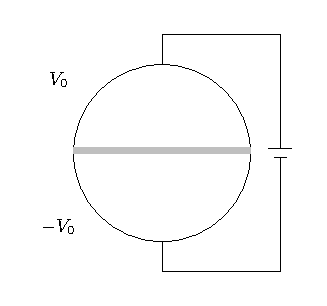
\includegraphics[scale=1]{Imagenes/Ejemplo_Esfera_03.eps}
    \caption{Dos hemisferios conductores cada uno con un potencial. El hemisferio superior tiene un rango para el ángulo polar $0 \leq \theta < \pi/2$ o $0 < \cos \theta \leq 1$, mientras que el hemisferio inferior tiene el rango $\pi/2 < \theta \leq \pi $ o $-1 \leq \cos \theta < 0$.}
    \label{fig_figura_esfera_03}
\end{figure}
\end{frame}
\begin{frame}
\frametitle{Problema a resolver}
\textbf{Queremos encontrar el potencial en puntos fuera de la esfera resultante}.
\end{frame}
\begin{frame}
\frametitle{Consideración importante}
Dado que el \textbf{\textcolor{cobalt}{potencial debe anularse en el infinito}}, \pause esperamos que el primer término en la ecuación (\ref{eq:ecuacion_26_29}) esté ausente, \pause es decir, debe de ocurrir que $A_{k} = 0$.
\end{frame}
\begin{frame}
\frametitle{Expresión de trabajo}
Para encontrar $B_{k}$, sustituimos $a$ por $r$ en la ec. (\ref{eq:ecuacion_26_29}), y sea $\cos \theta \equiv u$.
\\
\bigskip
\pause
 Entonces:
\begin{align*}
\psi (a, u) = \nsum_{k=0}^{\infty} \underbrace{\dfrac{B_{k}}{a^{k+1}}}_{\mbox{\large $\equiv c_{k}$}} \, P_{k} (u)
\end{align*}
\end{frame}
\begin{frame}
\frametitle{La función en la esfera}
Donde:
\pause
\begin{align*}
\psi (a, u) = \begin{cases}
- V_{0} & \mbox{ si } -1 \leq u < 0 \\[1em]
+ V_{0} & \mbox{ si } 0 < u \leq 1
\end{cases}
\end{align*}
\end{frame}
\begin{frame}
\frametitle{Obteniendo los coeficientes}
El cálculo de los coeficientes es idéntico al del ejemplo de las notas de trabajo. 
\\
\bigskip
\pause
Por lo tanto, $c_{k} = 0$ para $k$ par, además:
\pause
\begin{align*}
c_{2m+1} = \dfrac{B_{2m+1}}{a^{2m+2}} = (-1)^{m} \, \dfrac{(4 m + 3)(2 m)!}{2^{2m+1} (m + 1)! m!} \, V_{0}
\end{align*}
\end{frame}
\begin{frame}
\frametitle{Obteniendo los coeficientes}
Que despejando para los coeficientes $B_{2m+1}$:
\pause
\begin{align*}
B_{2m+1} = \dfrac{(-1)^{m} \, (4 m + 3)(2 m)!}{2^{2m+1} m! (m + 1)!} \, a^{2m+2} \, V_{0}
\end{align*}
\end{frame}
\begin{frame}
\frametitle{Solución al problema}
Una vez que se calcularon los coeficientes, el potencial queda dado por:
\pause
\begin{align}
\begin{aligned}
\psi (r, \theta) &= V_{0} \nsum_{m=0}^{\infty} (-1)^{m} \, \dfrac{(4 m + 3)(2 m)!}{2^{2m+1} m! (m + 1)!} \times \\[0.5em]
&\times \left( \dfrac{a}{r} \right)^{2m+2} \, P_{2m+1} (\cos \theta)
\end{aligned}
\label{eq:ecuacion:26_53}
\end{align}
\end{frame}

\section{Ejercicios a cuenta}
\frame[allowframebreaks]{\frametitle{Temas a revisar} \tableofcontents[currentsection, hideothersubsections]}
\subsection{Enunciados}

\begin{frame}
\frametitle{Ejercicio 1}
Una esfera conductora de calor de radio $a$ está compuesta por dos hemisferios con un espacio infinitesimal aislante entre ellos, como se muestra en la figura (\ref{fig:figura2}).
\end{frame}
\begin{frame}
\frametitle{Ejercicio 1}
\begin{figure}[H]
    \centering
   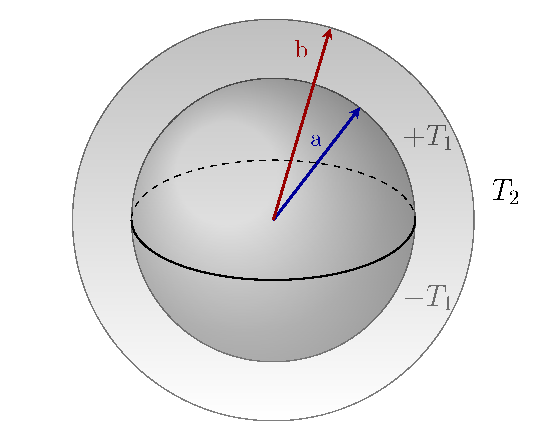
\includegraphics[scale=0.9]{Imagenes/esfera1.eps}
    \caption{Los hemisferios de la esfera interior se encuentran a diferentes temperatura.}
    \label{fig:figura2}
\end{figure}
\end{frame}
\begin{frame}
\frametitle{Ejercicio 1}
Las mitades superior e inferior de la esfera están en contacto con baños térmicos de temperaturas $+ T_{1}$ y $-T_{1}$, respectivamente.
\\
\bigskip
La esfera de radio $a$ está dentro de otra esfera conductora de calor de radio $b$ con una temperatura $T_{2}$.
\end{frame}
\begin{frame}
\frametitle{Ejercicio 1}
Calcula la temperatura:
\setbeamercolor{item projected}{bg=cobalt,fg=white}
\setbeamertemplate{enumerate items}{%
\usebeamercolor[bg]{item projected}%
\raisebox{1.5pt}{\colorbox{bg}{\color{fg}\footnotesize\insertenumlabel}}%
}
\begin{enumerate}
\item Dentro de la esfera interior,
\item En la región entre las dos esferas, y
\item Por fuera de la esfera exterior.
\end{enumerate}
\end{frame}
\begin{frame}
\frametitle{Ejercicio 2}
%Ref. Boas (20059 Chapter 12. Problems 10, 12)
Expande en términos de una serie con Polinomios de Legendre los siguientes polinomios:
\setbeamercolor{item projected}{bg=cobalt,fg=white}
\setbeamertemplate{enumerate items}{%
\usebeamercolor[bg]{item projected}%
\raisebox{1.5pt}{\colorbox{bg}{\color{fg}\footnotesize\insertenumlabel}}%
}
\begin{enumerate}
\item $f (x) = 3 \, x^{2} + x - 1$
\item $g (x) = x - x^{3}$
\end{enumerate}
\end{frame}

% \section{Ejercicio esfera aterrizada.}

% Veamos otro ejemplo de la solución de la ecuación de Laplace en coordenadas esféricas, consideremos una esfera conductora neutra puesta a tierra de radio $a$ colocada en un campo eléctrico originalmente uniforme $E_{0}$ que se supone que tiene una extensión infinita, como se muestra en la figura (\ref{fig:figura_esfera_aterrizada})).
% \begin{figure}[H]
%     \centering
%     \includegraphics[scale=0.4]{Imagenes/Esfera_Compo_Electrico.png}
%     \caption{El campo eléctrico en la vecindad de una esfera colocada en un campo uniforme externo cambiará, pero el campo alejado de la esfera permanecerá casi uniforme.}
%     \label{fig:figura_esfera_aterrizada}
% \end{figure}

% \textbf{Queremos encontrar el potencial electrostático en todas partes fuera de la esfera}.
% \par
% Eligiendo que el campo esté en la dirección $z$ positiva y colocando el centro de la esfera en el origen, tendremos un problema que presenta simetría azimutal. Por lo tanto, la solución general viene dada por la ec. (\ref{eq:ecuacion_26_29}). Los límites por fuera de la esfera consisten en la esfera misma así como en el infinito. El campo eléctrico en el infinito es el campo uniforme original, porque el campo debido a las cargas inducidas en la esfera desaparece en el infinito. El potencial de este campo (en el infinito) se puede deducir de:
% \begin{align*}
% \vb{E} &= E_{0} \, \vu{e}_{z} = - \grad{\Phi} \\[0.5em]
% \Rightarrow \hspace{0.2cm} E_{0} &= - \pdv{\Phi}{z}, \hspace{1cm} \pdv{\Phi}{x} = \pdv{\Phi}{y} = 0
% \end{align*}
% Por lo tanto, el potencial en el infinito es independiente de $x$ e $y$, y se puede escribir como:
% \begin{align*}
% \Phi (r, \theta) &= - E_{0} \, z = \\[0.5em]
% &= - E_{0} \, r \, \cos \theta = \\[0.5em]
% &= - E_{0} \, r \, P_{1} (\cos \theta) \hspace{1cm} \mbox{para } r \to \infty
% \end{align*}
% Por lo tanto, el potencial en el infinito es independiente de $x$ e $y$, y se puede escribir como:

%Ref. Butkov (1973) 9.8 Spherical Bessel Functions
\section{Polinomios asociados de Legendre}
\frame[allowframebreaks]{\frametitle{Temas a revisar} \tableofcontents[currentsection, hideothersubsections]}
\subsection{Ecuación  de onda}

\begin{frame}
\frametitle{Uso de los polinomios asociados de Legendre}
La principal utilidad de los polinomios asociados de Legendre es en la expansión de funciones definidas en la superficie de una esfera.
\\
\bigskip
\pause
Veamos el caso con la función de onda.
\end{frame}
\begin{frame}
\frametitle{Función de onda}
Para cada frecuencia fija \pause (puede ser una eigenfrecuencia determinada a partir de la ecuación radial) \pause $\omega = k \, c$ le corresponde un modo:
\pause
\begin{align*}
\varphi_{k} (\vb{r}, t) = \psi_{k} (\vb{r}) \, \exp(- i \omega t)
\end{align*}
\end{frame}
\begin{frame}
\frametitle{Ecuación de Helmholtz}
Donde $\psi_{k} (\vb{r})$ satisface la ecuación de Helmholtz:
\pause
\begin{align*}
\laplacian{\psi_{k}} + k^{2} \, \psi_{k} = 0
\end{align*}
\end{frame}
\begin{frame}
\frametitle{Resolviendo la ecuación}
Para resolver la ecuación, propongamos una separación de variables del tipo:
\pause
\begin{align*}
\psi_{k} (r, \theta, \phi) = R (r) \, Y (\theta, \phi)
\end{align*}
\pause
que nos lleva a:
\pause
\begin{eqnarray*}
\begin{aligned}
\dv{r} \bigg( r^{2} \, \dv{R}{r} \bigg) &+ \big( k^{2} \, r^{2} + \lambda \big) \, R = 0 \\[0.5em] \pause
\dfrac{1}{\sin \theta} \, \pdv{\theta} \bigg( \sin \theta \, \pdv{Y}{\theta} \bigg) &+ \dfrac{1}{\sin^{2} \theta} \, \pdv[2]{Y}{\phi} + \lambda \, Y = 0
\end{aligned}
\end{eqnarray*}
\end{frame}
\begin{frame}
\frametitle{El tipo de eigenvalor}
El eigenvalor $\lambda$ se determinará a partir de la segunda ecuación, \pause tomemos en cuenta que:
\pause
\setbeamercolor{item projected}{bg=olive,fg=white}
\setbeamertemplate{enumerate items}{%
\usebeamercolor[bg]{item projected}%
\raisebox{1.5pt}{\colorbox{bg}{\color{fg}\footnotesize\insertenumlabel}}%
}
\begin{enumerate}[<+->]
\item $Y (\theta, \phi)$ debe de ser finito para $0 \leq \theta \leq \pi$ y$0 \leq \phi \leq 2 \pi$
\item Tendremos eigenfunciones $Y_{\lambda} (\theta, \phi)$ correspondientes a esos eigenvalores.
\end{enumerate}
\end{frame}
\begin{frame}
\frametitle{Solución completa}
Entonces, la función completa $\phi_{k} (\vb{r})$ se puede expresar por una superposición del tipo:
\pause
\begin{align*}
\psi_{k} (\vb{r}) = \nsum_{\lambda} C_{\lambda} \, R_{\lambda} (r) \, Y_{\lambda} (\theta, \phi)
\end{align*}
\pause
\textbf{Nota: } La suma sobre $\lambda$ debe de considerarse como simbólica, ya que aún no hemos explorado la estructura del espectro de $\lambda$: ya sea continuo o discreto, ya sea que tenga o no degeneración.
\end{frame}
\begin{frame}
\frametitle{Eigenvalores permitidos}
Para establecer los valores permitidos de $\lambda$, completamos la separación de variables, haciendo:
\pause
\begin{align*}
Y (\theta, \phi) = \Theta (\theta) \, \Phi (\phi)
\end{align*}
\end{frame}
\begin{frame}
\frametitle{Nueva separación de variables}
Lo que nos lleva a las ecuaciones:
\pause
\begin{eqnarray*}
\begin{aligned}
\dv{\theta} \bigg( \sin \theta \, \dv{\Theta}{\theta} \bigg) + \bigg( - \sin \theta \lambda + \dfrac{\lambda_{1}}{\sin \theta} \bigg) \, \Theta &= 0 \\[0.5em] \pause
\dv[2]{\Phi}{\phi} - \lambda_{1} \, \Phi &= 0
\end{aligned}
\end{eqnarray*}
las cuales ya hemos resuelto anteriormente.
\end{frame}
\begin{frame}
\frametitle{Propiedad de los eigenvalores}
Sabemos que el espectro de $\lambda_{1}$ es discreto, sea:
\begin{align*}
\lambda_{1} = - m^{2} ~ (m = 0, 1, 2, \ldots)
\end{align*}
\end{frame}
\begin{frame}
\frametitle{Definiendo las eigenfunciones}
Las eigenfunciones pueden definirse de la siguiente manera.
\pause
\\
\noindent
Para $m = 0$:
\pause
\begin{align*}
\Phi_{0} (\phi) = 1
\end{align*}
\pause
para $m \neq 0$:
\begin{align*}
\Phi_{m} (\phi) = \begin{cases}
\cos m \phi & \mbox{o bien} \\
\sin m \phi
\end{cases}
\end{align*}
\end{frame}
\begin{frame}
\frametitle{Ortogonalidad de las funciones}
Estas funciones son ortogonales entre sí y las integrales de normalización son:
\pause
\begin{eqnarray*}
\begin{aligned}
\scaleint{6ex}_{\bs 0}^{2 \pi} \big[ \Phi_{0} (\phi) \big]^{2} \dd{\phi} &= 2 \, \pi \\[0.5em] \pause
\scaleint{6ex}_{\bs 0}^{2 \pi} \cos^{2} m \, \phi \dd{\phi} &= \pi \\[0.5em] \pause
\scaleint{6ex}_{\bs 0}^{2 \pi} \sin^{2} m \, \phi \dd{\phi} &= \pi
\end{aligned}
\end{eqnarray*}
\end{frame}
\begin{frame}
\frametitle{Normalización de las funciones}
Es conveniente en este momento tener esas eigenfunciones \textocolor{blue-violet}{normalizadas a la unidad}, \pause para ello las multiplicamos por las constantes apropiadas para que todas las integrales de normalización sean iguales a la unidad.
\end{frame}
\begin{frame}
\frametitle{Normalización de las funciones}
Esta condición define las funciones normalizadas:
\pause
\begin{eqnarray*}
\begin{aligned}
&\Phi_{0} (\phi) = \dfrac{1}{\sqrt{2 \pi}} \hspace{0.3cm} (m = 0) \\[0.5em] \pause
&\left. \begin{aligned}
\Phi_{m}^{(+)} (\phi) &= \dfrac{1}{\sqrt{\pi}} \, \cos m \, \phi \\[0.5em] \pause
\Phi_{m}^{(-)} (\phi) &= \dfrac{1}{\sqrt{\pi}} \, \sin m \, \phi
\end{aligned} \right\}
(m \neq 0)
\end{aligned}
\end{eqnarray*}
\pause
donde el símbolo $(+)$ o $(-)$ nos recuerda que esas funciones son pares o impares con respecto al intercambio $\phi \leftrightarrow - \phi$.
\end{frame}
\begin{frame}
\frametitle{Espectro de los eigenvalores}
En cuanto a las funciones $\Theta$ se refiere, \pause sabemos que el espectro de $\lambda$ es también discreto, con:
\pause
\begin{align*}
\lambda = - \ell (\ell + 1) \hspace{0.5cm} \ell = 0, 1, 2, \ldots
\end{align*}
pero para cualquier $m$ dado, se tiene que $\ell \geq m$.
\end{frame}
\begin{frame}
\frametitle{Los polinomios asociados de Legendre}
Las soluciones de la ecuación con $\Theta$ son los polinomios asociados de Legendre:
\begin{align*}
P_{\ell}^{m} (\cos \theta)
\end{align*}
\end{frame}
\begin{frame}
\frametitle{Los $P_{n}^{m} (x)$}
\begin{align*}
\begin{aligned}
P_{0}^{0} (x) &= 1, \\[6pt]
P_{1}^{0} (x) &= x, &
P_{1}^{1} (x) &= -\sqrt{1 - x^{2}}, \\[6pt]
P_{2}^{0} (x) &= \tfrac{1}{2}(3 x^{2} - 1), &
P_{2}^{1} (x) &= -3 x\sqrt{1 - x^{2}}, \\[6pt]
P_{2}^{2} (x) &= 3(1 - x^{2})
\end{aligned}
\end{align*}
\end{frame}
\begin{frame}
\frametitle{Los $P_{n}^{m} (x)$}
\begin{align*}
\begin{aligned}
P_{3}^{0} (x) &= \tfrac{1}{2}(5 x^{3} - 3 x) \\[6pt]
P_{3}^{1} (x) &= -\tfrac{3}{2}(5 x^{2} - 1) \sqrt{1 - x^2}, \\[6pt] 
P_{3}^{2} (x) &= 15 x(1 - x^{2}), \\[6pt]
P_{3}^{3} (x) &= -15(1 - x^{2})^{3/2}
\end{aligned}
\end{align*}
\end{frame}
\begin{frame}
\frametitle{Los $P_{n}^{m} (\cos \theta)$}
\begin{align*}
\begin{aligned}
P_{0}^{0} (\cos \theta) &= 1, \\[6pt]
P_{1}^{0} (\cos \theta) &= \cos \theta, \\[6pt]
P_{1}^{1} (\cos \theta) &= -\sin \theta, \\[6pt]
P_{2}^{0} (\cos \theta) &= \tfrac{1}{2} (3 \cos^{2} \theta - 1), \\[6pt]
P_{2}^{1} (\cos \theta) &= -3 \cos \theta\,\sin \theta, \\[6pt]
P_{2}^{2} (\cos \theta) &= 3 \sin^{2} \theta
\end{aligned}
\end{align*}
\end{frame}
\begin{frame}
\frametitle{Los $P_{n}^{m} (\cos \theta)$}
\begin{align*}
\begin{aligned}
P_{3}^{0} (\cos \theta) &= \tfrac{1}{2}(5 \cos^{3} \theta - 3 \cos \theta), \\[6pt]
P_{3}^{1} (\cos \theta) &= -\tfrac{3}{2}(5 \cos^{2} \theta - 1) \sin \theta, \\[6pt]
P_{3}^{2} (\cos \theta) &= 15 \cos \theta\,\sin^{2} \theta, \\[6pt]
P_{3}^{3} (\cos \theta) &= -15 \sin^{3} \theta
\end{aligned}
\end{align*}
\end{frame}
\begin{frame}
\frametitle{Gráfica de los $P_{n}^{m} (x)$}
\begin{figure}
  \centering
  \includegraphics[width=0.9\linewidth]{Imagenes/plot_Asociados_Legendre_01.pdf}
\end{figure}
\end{frame}
\begin{frame}
\frametitle{Gráfica de los $P_{n}^{m} (x)$}
\begin{figure}
  \centering
  \includegraphics[width=0.9\linewidth]{Imagenes/plot_Asociados_Legendre_02.pdf}
\end{figure}
\end{frame}
\begin{frame}
\frametitle{Gráfica de los $P_{n}^{m} (x)$}
\begin{figure}
  \centering
  \includegraphics[width=0.9\linewidth]{Imagenes/plot_Asociados_Legendre_03.pdf}
\end{figure}
\end{frame}
\begin{frame}
\frametitle{Gráfica de los $P_{n}^{m} (x)$}
\begin{figure}
  \centering
  \includegraphics[width=0.9\linewidth]{Imagenes/plot_Asociados_Legendre_04.pdf}
\end{figure}
\end{frame}
\begin{frame}
\frametitle{Normalización de los $P_{\ell}^{m}$}
Es conveniente normalizarlos a la unidad también, definiendo entonces:
\pause
\begin{align*}
\Theta_{\ell}^{m} (\cos \theta) = \sqrt{\dfrac{2 \ell + 1}{2} \, \dfrac{(\ell - m)!}{(\ell + m)!}} \, P_{\ell}^{m} (\cos \theta)
\end{align*}
\end{frame}
\begin{frame}
\frametitle{Normalizando los $P_{\ell}^{m}$}
Por lo que:
\pause
\begin{eqnarray*}
\begin{aligned}
&\scaleint{6ex}_{\bs 0}^{\pi} \big[ \Theta_{\ell}^{m} (\cos \theta) \big]^{2} \sin \theta \dd{\theta} = \\[0.5em] \pause
&=\dfrac{2 \ell + 1}{2} \, \dfrac{(\ell - m)!}{(\ell + m)!} \, \scaleint{6ex}_{\bs -1}^{+1} \big[ P_{\ell}^{m}  (x) \big]^{2} \dd{x} = \pause 1
\end{aligned}
\end{eqnarray*}
\end{frame}
\begin{frame}
\frametitle{Problema de eigenvalores}
Ahora debería de quedar claro que la ecuación de eigenvalores:
\pause
\begin{align*}
\dfrac{1}{\sin \theta} \, \pdv{\theta} \bigg( \sin \theta \, \pdv{Y}{\theta} \bigg) &+ \dfrac{1}{\sin^{2} \theta} \, \pdv[2]{Y}{\phi} + \lambda \, Y = 0
\end{align*}
\pause
tiene los eigenvalores:
\pause
\begin{align*}
\lambda = - \ell (\ell + 1) \hspace{0.4cm} \ell = 0, 1, 2, \ldots
\end{align*}
\end{frame}
\begin{frame}
\frametitle{Degeneración en las eigenfunciones}
Los eigenvalores son, sin embargo, \pause \emph{degenerados} (excepto si $\ell = 0)$, \pause por que para cada valor fijo de $\ell$, se tiene varias eigenfunciones:
\pause
\begin{eqnarray*}
\begin{aligned}
&\Theta_{\ell}^{0} (\cos \theta) \, \Phi_{0} (\phi) \\[0.5em] \pause
&\Theta_{\ell}^{1} (\cos \theta) \, \Phi_{1}^{(+)} (\phi) \hspace{0.7cm} \Theta_{\ell}^{1} (\cos \theta) \, \Phi_{1}^{(-)} (\phi) \\[0.5em] \pause
&\Theta_{\ell}^{2} (\cos \theta) \, \Phi_{2}^{(+)} (\phi) \hspace{0.7cm} \Theta_{\ell}^{2} (\cos \theta) \, \Phi_{2}^{(-)} (\phi) \\[0.5em] \pause
&{} \hspace{0.3cm} \vdots
\end{aligned}
\end{eqnarray*}
y así sucesivamente.
\end{frame}
\begin{frame}
\frametitle{Eigenfunciones degeneradas}
Hasta llegar a:
\pause
\begin{align*}
\Theta_{\ell}^{\ell} (\cos \theta) \, \Phi_{\ell}^{(+)} (\phi) \hspace{0.5cm} \Theta_{\ell}^{\ell} (\cos \theta) \, \Phi_{\ell}^{(-)} (\phi)
\end{align*}
\pause
Para cada valor de $\ell$ le corresponden $(2 \ell + 1)$ eigenfunciones, teniendo entonces un orden de degeneración de $(2 \ell + 1)$.
\end{frame}
\begin{frame}
\frametitle{Soluciones fundamentales}
Definimos las soluciones fundamentales de la EDP (sujeta a las CDF apropiadas):
\pause
\begin{align*}
\dfrac{1}{\sin \theta} \, \pdv{\theta} \bigg( \sin \theta \, \pdv{Y}{\theta} \bigg) &+ \dfrac{1}{\sin^{2} \theta} \, \pdv[2]{Y}{\phi} + \ell (\ell + 1) \, Y = 0
\end{align*}
\end{frame}
\begin{frame}
\frametitle{Soluciones fundamentales}
Por medio de las expresiones:
\pause
\begin{eqnarray*}
&Y_{\ell 0} (\theta, \phi) = \sqrt{\dfrac{2 \ell + 1}{4 \pi}} \, P_{\ell} (\cos \theta) \hspace{0.3cm} (m = 0)
\end{eqnarray*}
\end{frame}
\begin{frame}
\frametitle{Soluciones fundamentales}
\begin{eqnarray*}
\begin{aligned}
&\left. \begin{aligned}
&Y_{\ell m}^{(+)} (\theta, \phi) = \Theta_{\ell}^{m} (\cos \theta) \, \Phi_{m}^{(+)} (\phi) = \\[0.5em] \pause
&= \sqrt{\dfrac{2 \ell + 1}{2 \pi} \, \dfrac{(\ell - m)!}{(\ell + m)!}} \, P_{\ell}^{m} (\cos \theta) \, \cos m \phi \\[0.5em] \pause
&Y_{\ell m}^{(-)} (\theta, \phi) = \Theta_{\ell}^{m} (\cos \theta) \, \Phi_{m}^{(-)} (\phi) = \\[0.5em] \pause
&= \sqrt{\dfrac{2 \ell + 1}{2 \pi} \, \dfrac{(\ell - m)!}{(\ell + m)!}} \, P_{\ell}^{m} (\cos \theta) \, \sin m \phi
\end{aligned} \right\}
(m \neq 0)
\end{aligned}
\end{eqnarray*}
\end{frame}
\begin{frame}
\frametitle{Nombrando a las soluciones}
Estas soluciones son los armónicos esféricos, en la definición clásica.
\\
\bigskip
\pause
De manera contraria en la definición de los armónicos esféricos en la mecánica cuántica, donde $\cos m \phi$ y $\sin m \phi$ se descartan en favor de $\exp(i m \phi)$ y $\exp(-i m \phi)$.
\end{frame}
\begin{frame}
\frametitle{La solución en series}
Se sigue entonces que la expresión en series para $\psi_{k} (\vb{r})$ es del tipo:
\pause
\begin{align*}
\psi_{k} (\vb{r}) = \nsum_{\lambda} C_{\lambda} \, R_{\lambda} (r) \, Y_{\lambda} (\theta, \phi)
\end{align*}
\end{frame}
\begin{frame}
\frametitle{Solución en series}
Es de la forma:
\pause
\begin{align*}
\psi_{k} (\vb{r}) &= \nsum_{\ell=0}^{\infty} R_{\ell} (r) \bigg[ C_{\ell 0} \, Y_{\ell 0} (\theta, \phi) + \\[0.5em]
&+ \nsum_{m=1}^{\ell} \bigg( C_{\ell m}^{(+)} \, Y_{\ell m}^{(+)} (\theta, \phi) + C_{\ell m}^{(-)} \, Y_{\ell m}^{(-)} (\theta, \phi) \bigg) \bigg]
\end{align*}
\end{frame}
\begin{frame}
\frametitle{Analizando la solución}
Supongamos que $r$ está fijo, \pause entonces $\psi_{k} (\vb{r})$ se convierte en una función solo de $\theta$ y $\phi$, por lo que estaremos tratando con una expresión del tipo:
\pause
\begin{align*}
f (\theta, \phi) &= \nsum_{\ell=0}^{\infty} \bigg[ A_{\ell 0} \, Y_{\ell 0} (\theta, \phi) + \\[0.5em]
&+ \nsum_{m=1}^{\ell} \bigg( A_{\ell m}^{(+)} \, Y_{\ell m}^{(+)} (\theta, \phi) + A_{\ell m}^{(-)} \, Y_{\ell m}^{(-)} (\theta, \phi) \bigg) \bigg]
\end{align*}
\end{frame}
\begin{frame}
\frametitle{Solución válida}
Esta expansión en serie es válida para una función arbitraria $f (\theta, \phi)$, sujeta a las condiciones habituales similares para las series de Fourier, series de Fourier-Legendre, series de Fourier-Bessel, etc.
\end{frame}
\begin{frame}
\frametitle{Reecuperando los coeficientes}
Los coeficientes de la expansión se obtienen multiplicando $f (\theta, \phi)$ por el correspondiente armónico esférico y por el factor $\sin \theta$, para luego integrar sobre los ángulos:
\pause
\begin{eqnarray*}
\begin{aligned}
A_{\ell 0} &= \scaleint{6ex}_{\bs 0}^{\pi} \scaleint{6ex}_{\bs 0}^{2 \pi} f (\theta, \phi) \, Y_{\ell 0} (\theta, \phi) \, \sin \theta \dd{\theta} \dd{\phi} \hspace{0.5cm} (m = 0) \\[0.5em] \pause
A_{\ell m}^{(\pm)} &= \scaleint{6ex}_{\bs 0}^{\pi} \scaleint{6ex}_{\bs 0}^{2 \pi} f (\theta, \phi) \, Y_{\ell 0}^{(\pm)} (\theta, \phi) \, \sin \theta \dd{\theta} \dd{\phi} \hspace{0.5cm} (m \neq 0)
\end{aligned}
\end{eqnarray*}
\end{frame}
\begin{frame}
\frametitle{Observación importante}
El factor $\sin \theta$ que se necesita para la ortogonalidad de las funciones $P_{\ell}^{m}$, tiene la siguiente interpretación geométrica: Un ángulo sólido se define por:
\pause
\begin{align*}
\dd{\Omega} = \dfrac{\dd{S}}{r^{2}}
\end{align*}
donde $\dd{S}$ es el elemento de área de una esfera de radio $r$.
\end{frame}
\begin{frame}
\frametitle{Elemento de área en coord. esféricas}
En el sistema esférico:
\pause
\begin{align*}
\dd{S} = r \, \dd{\theta} \, r \, \sin \theta \dd{\phi}
\end{align*}
\pause
Tal que:
\pause
\begin{align*}
\dd{\Omega} = \sin \theta \dd{\theta} \dd{\phi}
\end{align*}
y las integrales citadas anteriormente pueden considerarse integrales sobre el ángulo sólido.
\end{frame}
\begin{frame}
\frametitle{Integrales sobre el ángulo sólido}
Y escribirse simbólicamente como:
\pause
\begin{eqnarray*}
\begin{aligned}
A_{\ell 0} &= \scaleint{6ex}_{\Omega} f (\Omega) \, Y_{\ell 0} (\Omega) \dd{\Omega} \hspace{0.5cm} (m = 0) \\[0.5em] \pause
A_{\ell m}^{\pm} &= \scaleint{6ex}_{\Omega} f (\Omega) \, Y_{\ell m}^{\pm} (\Omega) \dd{\Omega} \hspace{0.5cm} (m \neq 0)
\end{aligned}
\end{eqnarray*}
\end{frame}

\section{Las funciones esféricas de Bessel}
\frame[allowframebreaks]{\frametitle{Temas a revisar} \tableofcontents[currentsection, hideothersubsections]}
\subsection{Ec. Onda y de Helmholtz}

\begin{frame}
\frametitle{La ec. de onda}
Continuemos revisando las EDP de onda y de Helmholtz en coordenadas esféricas. \pause Sabemos que la ecuación radial es de la forma:
\pause
\begin{align*}
\dv{r} \bigg( r^{2} \dv{R}{r} \bigg) + \big[ k^{2} r^{2} {-} \ell (\ell {+} 1) \big] R = 0 \hspace{0.5cm} \ell = 0, 1, \ldots
\end{align*}
\end{frame}
\begin{frame}
\frametitle{Haciendo un cambio de variable}
Si hacemos el cambio de variable $x = k \, r$, $y (x) \equiv R (r)$, la ecuación se reduce a:
\pause
\begin{align*}
x^{2} \, \dv[2]{y}{x} + 2 \, x \, \dv{y}{x} + \big[ x^{2} - \ell (\ell + 1) \big] \, y = 0
\end{align*}
\end{frame}
\begin{frame}
\frametitle{Soluciones a la ecuación}
Las soluciones de esta ED se conocen como:
\pause
\setbeamercolor{item projected}{bg=olive,fg=white}
\setbeamertemplate{enumerate items}{%
\usebeamercolor[bg]{item projected}%
\raisebox{1.5pt}{\colorbox{bg}{\color{fg}\footnotesize\insertenumlabel}}%
}
\begin{enumerate}[<+->]
\item Las \emph{funciones esféricas de Bessel}: $j_{\ell} (x)$
\item Las funciones \emph{esféricas de Neumann}: $n_{j} (x)$
\end{enumerate}
\pause
de orden $\ell$.
\end{frame}
\begin{frame}
\frametitle{Origen del nombre de las funciones}
La razón de darles ese nombre es debido al cambio de variable:
\pause
\begin{align*}
y (x) = \dfrac{u (x)}{\sqrt{x}}
\end{align*}
\end{frame}
\begin{frame}
\frametitle{Expresión modificada}
Que reduce la ecuación a la forma:
\pause
\begin{align*}
\dv[2]{u}{x} + \dfrac{1}{x} \dv{u}{x} + \bigg[ 1 - \dfrac{\big( \ell + \frac{1}{2} \big)}{x^{2}} \bigg] \, u = 0 \hspace{0.5cm} \ell = 0, 1, 2, \ldots
\end{align*}
\pause
que reconocemos es la ED de Bessel de orden $\ell + 1/2$.
\end{frame}
\begin{frame}
\frametitle{Soluciones de la ED}
Se sigue entonces que las soluciones de la ED inicial, pueden escribirse de la forma:
\pause
\begin{align*}
y (x) = C_{1} \, \dfrac{J_{\ell+1/2} (x)}{\sqrt{x}} + C_{2} \, \dfrac{J_{-\ell-1/2} (x)}{\sqrt{x}}
\end{align*}
\end{frame}
\begin{frame}
\frametitle{Solución finita en el origen}
Si la función de Bessel esférica $j_{\ell} (x)$ se define como una solución finita en $x = 0$, \pause se sigue que debe ser un múltiplo de $J_{\ell+1/2} (x) / \sqrt{x}$.
\\
\bigskip
\pause
El factor de proporcionalidad generalmente se elige para que sea $\sqrt{\pi/2}$, por lo tanto:
\pause
\begin{align*}
j_{\ell} (x) = \sqrt{\dfrac{\pi}{2 x}} \, J_{\ell+1/2} (x)
\end{align*}
\end{frame}
\begin{frame}
\frametitle{Relación entre funciones}
La relación de las $j_{\ell} (x)$ con las funciones de Bessel, nos permiten expresar las $j_{\ell} (x)$ en términos de $j_{0} (x)$. \pause De la expresión:
\pause
\begin{align*}
J_{\mu+1} (x) = - x^{\mu} \, \dv{x} \bigg[ \dfrac{J_{\mu} (x)}{x^{\mu}} \bigg]
\end{align*}
\end{frame}
\begin{frame}
\frametitle{Nuevo cambio de variable}
Que entonces, al hacer $\mu = \ell + 1/2$ y dividiendo entre $x^{\ell+3/2}$, se tiene:
\pause
\begin{eqnarray*}
\begin{aligned}
\dfrac{J_{\ell+3/2} (x)}{x^{\ell+3/2}} &= - \dfrac{1}{x} \, \dv{x} \bigg[ \dfrac{J_{\ell+1/2} (x)}{x^{\ell+1/2}} \bigg] \\[0.5em] \pause
\mbox{o } \hspace{0.3cm} \dfrac{j_{\ell+1} (x)}{x^{\ell+1}} &= - \dfrac{1}{x} \dv{x} \bigg[ \dfrac{j_{\ell} (x)}{x^{\ell}} \bigg]
\end{aligned}
\end{eqnarray*}
\end{frame}
\begin{frame}
\frametitle{Valores con $\ell$}
Comenzando con $\ell = 0$ y ocupando esta expresión $\ell$ veces, se obtiene:
\pause
\begin{align*}
j_{\ell} (x) = x^{\ell} \bigg( - \dfrac{1}{x} \, \dv{x} \bigg)^{\ell} \, j_{0} (x) \hspace{0.5cm} \ell = 1, 2, \ldots 
\end{align*}
\end{frame}
\begin{frame}
\frametitle{Expresión para valores de $j_{0}$}
Esta expresión únicamente define todas las $j$ funciones una vez que $j_{0}$ se elige. Nuestra ecuación para $\ell = 0$ es entonces:
\pause
\begin{align*}
\dv[2]{y}{x} + \dfrac{2}{x} \, \dv{y}{x} + y = 0
\end{align*}
\end{frame}
\begin{frame}
\frametitle{Resolviendo la ED}
Resolviendo esta ecuación (ya sea por Frobenius o por otro método), \pause encontramos que las funciones $\sin x /x$ y $\cos x /x$ están entre las soluciones.
\\
\bigskip
\pause
Es común definir:
\pause
\begin{align*}
j_{0} (x) = \dfrac{\sin x}{x}
\end{align*}
\end{frame}
\begin{frame}
\frametitle{Comparando el resultado}
En comparación con $J_{1/2}$, se tiene:
\pause
\begin{align*}
j_{0} (x) = \sqrt{\dfrac{\pi}{2 x}} \, J_{1/2} (x)
\end{align*}
que explica el factor $\sqrt{\pi / 2}$.
\end{frame}
\begin{frame}
\frametitle{Segunda  solución}
Las funciones esféricas de Neumann $n_{\ell} (x)$ se generan de manera similar a partir de $n_{0} (x)$ por medio de:
\pause
\begin{align*}
n_{\ell} (x) = x^{\ell} \bigg( - \dfrac{1}{x} \, \dv{x} \bigg)^{\ell} \, n_{0} (x) \hspace{0.5cm} \ell = 1, 2, \ldots
\end{align*}
\end{frame}
\begin{frame}
\frametitle{Definición de $n_{0}$}
Siendo común definir:
\pause
\begin{align*}
n_{0} (x) = - \dfrac{\cos x}{x} = \sqrt{\dfrac{\pi}{2 x}} \, J_{-1/2} (x)
\end{align*}
\end{frame}
\begin{frame}
\frametitle{Algunas funciones $j_{\ell} (x)$}
A continuación se presenta una lista con algunas funciones $j_{\ell} (x)$:
\pause
\begin{eqnarray*}
\begin{aligned}
j_{0} (x) &= \dfrac{\sin x}{x} \\[0.5em] \pause
j_{1} (x) &= \dfrac{\sin x}{x^{2}} - \dfrac{\cos x}{x} \\[0.5em] \pause
j_{2} (x) &= \bigg( \dfrac{3}{x^{3}} - \dfrac{1}{x} \bigg) \, \sin x - \dfrac{3}{x^{2}} \, \cos x \\[0.5em] \pause
j_{3} (x) &= \bigg( \dfrac{15}{x^{4}} - \dfrac{6}{x^{2}} \bigg) \, \sin x - \bigg( \dfrac{15}{x^{3}} - \dfrac{1}{x} \bigg) \, \cos x 
\end{aligned}
\end{eqnarray*}
\end{frame}
\begin{frame}
\frametitle{Gráfica de las $j_{\ell} (x)$}
\begin{figure}[H]
    \centering
    \includegraphics[width=0.9\linewidth]{Imagenes/Plot_Esfericas_Bessel.pdf}
\end{figure}
\end{frame}
\begin{frame}
\frametitle{Algunas funciones $n_{\ell} (x)$}
En la siguiente lista ahora presentamos algunas funciones $n_{\ell} (x)$:
\pause
\begin{eqnarray*}
\begin{aligned}
n_{0} (x) &= - \dfrac{\cos x}{x} \\[0.5em] \pause 
n_{1} (x) &= - \dfrac{\cos x}{x^{2}} - \dfrac{\sin x}{x} \\[0.5em] \pause 
n_{2} (x) &= - \bigg( \dfrac{3}{x^{2}} - \dfrac{1}{x} \bigg) \, \cos x - \dfrac{3}{x^{2}} \, \sin x \\[0.5em] \pause 
n_{3} (x) &= - \bigg( \dfrac{15}{x^{4}} - \dfrac{6}{x^{2}} \bigg) \, \cos x - \bigg( \dfrac{15}{x^{3}} - \dfrac{1}{x} \bigg) \, \sin x
\end{aligned}
\end{eqnarray*}
\end{frame}
\begin{frame}
\frametitle{Observación importante}
Las funciones esféricas de Bessel están relacionadas con las funciones de Neumann, por la expresión:
\pause
\begin{align*}
n_{\ell} = \sqrt{\dfrac{\pi}{2 x}} \, N_{l+1/2} (x)
\end{align*}
Es un buen ejercicio demostrar que $N_{\ell+1/2} (x)$ es proporcional a $J_{-\ell-1/2} (x)$, \pause sin embargo, esto es cierto solo si $\ell$ es un número entero.
\end{frame}
\begin{frame}
\frametitle{Gráfica de las $n_{\ell} (x)$}
\begin{figure}[H]
    \centering
    \includegraphics[width=0.9\linewidth]{Imagenes/Plot_Esfericas_Neumann.pdf}
\end{figure}
\end{frame}

\section{Ejercicio}
\frame[allowframebreaks]{\frametitle{Temas a revisar} \tableofcontents[currentsection, hideothersubsections]}
\subsection{Ondas estacionarias}

\begin{frame}
\frametitle{Enunciado del ejercicio}
Dentro de una cavidad esférica de radio $a$ se generan ondas sonoras.
\\
\bigskip
\pause
Se desea investigar los patrones de ondas estacionarias dentro de la cavidad y sus frecuencias.
\end{frame}
\begin{frame}
\frametitle{Comenzando la solución}
El problema se puede formular en términos del potencial de velocidad que debe satisfacer la ecuación de onda:
\pause
\begin{align*}
\laplacian{\varphi} - \dfrac{1}{c^{2}} \, \pdv[2]{\varphi}{t} = 0
\end{align*}
\pause
Se supone que la fuente del sonido se elimina en $t = 0$ y se deja que el aire en la cavidad vibre libremente.
\end{frame}
\begin{frame}
\frametitle{Condiciones de frontera}
El problema está sujeto a la CDF:
\pause
\begin{align*}
\pdv{\varphi}{r} \eval_{r = a} = 0
\end{align*}
\end{frame}
\begin{frame}
\frametitle{Tipo de soluciones}
Estamos buscando soluciones de la forma:
\pause
\begin{align*}
\varphi_{k} (\vb{r},  t) = \psi_{k} (\vb{r}) \, \exp(-i \omega t) \hspace{0.7cm} (\omega = k \, c)
\end{align*}
\pause
tal que $\psi_{k} (\vb{r},  t)$ deba satisfacer:
\pause
\begin{align*}
\laplacian{\psi}_{k} + k^{2} \, \psi_{k} = 0 \hspace{0.4cm} \mbox{y} \hspace{0.4cm} \pdv{\psi_{k}}{r} \eval_{r = a} = 0 
\end{align*}
\end{frame}
\begin{frame}
\frametitle{Uso de los resultados anteriores}
De los resultados obtenidos previamente en este material, se tiene que:
\pause
\begin{align*}
&\psi_{k} (\vb{r}) = \nsum_{\ell=0}^{\infty} R_{\ell} (r) \bigg[ C_{\ell 0} \, Y_{\ell 0} (\theta, \phi) + \\[0.5em]
&+ \nsum_{m=0}^{\ell} \bigg( C_{\ell m}^{(+)} \, Y_{\ell m}^{(+)} (\theta, \phi) + C_{\ell m}^{(-)} \, Y_{\ell m}^{(-)} (\theta, \phi) \bigg) \bigg]
\end{align*}
donde los $Y_{\ell m}$ son los armónicos esféricos.
\end{frame}
\begin{frame}
\frametitle{La ecuación radial}
Las funciones $R (r)$ deben de cumplir con la EDO:
\pause
\begin{align*}
\dv{r} \bigg( r^{2} \dv{R_{\ell}}{r} \bigg) &+ \big[ k^{2} r^{2} {-} \ell (\ell + 1) \big] R_{\ell} = 0 \\[0.5em]
&\ell = 0, 1, 2, \ldots
\end{align*}
\end{frame}
\begin{frame}
\frametitle{Solución general a la ec. radial}
La solución general de esta ecuación es del tipo:
\pause
\begin{align*}
R_{\ell} (r) = A_{\ell} \, j_{\ell} (k r) + B_{\ell} \, n_{\ell} (k r) 
\end{align*}
\end{frame}
\begin{frame}
\frametitle{Congruencia con la física}
Ya que la función $n_{\ell} (k r)$ no es finita en $r = 0$, \pause debe de descartarse haciendo que $B_{\ell} = 0$.
\\
\bigskip
\pause
Los valores permitidos de $k$ están determinados por la CDF, lo que se reduce a:
\begin{align*}
\dv{r} j_{\ell} (k r) \eval_{r=a} = 0
\end{align*}
\end{frame}
\begin{frame}
\frametitle{Raíces de la función especial}
Las raíces de $\dv*{x} j_{\ell} (x)$ se pueden encontrar en tablas o mediante el uso de software matemático.
\pause
\begin{table}[H]
\centering
\large
\renewcommand{\arraystretch}{0.9}
\begin{tabular}{c c c}
$\ell$ & $n$ & $\alpha_{\ell n}$ \\ \hline
$0$ & $1$ & $0.0000$ \\ \hline
$1$ & $1$ & $0.6626$ \\ \hline
$2$ & $1$ & $1.0638$ \\ \hline
$0$ & $2$ & $1.4303$ \\ \hline
$3$ & $1$ & $1.4369$ \\ \hline
\end{tabular}
\end{table}
\end{frame}
\begin{frame}
\frametitle{Valores de $k$}
Los correspondientes valores de $k$ para nuestro problema, son los dados por:
\pause
\begin{align*}
k_{\ell n} = \dfrac{\pi \alpha_{\ell n}}{a}
\end{align*}
\pause
y las correspondientes frecuencias están dadas de modo que:
\begin{align*}
\omega_{\ell n} = \dfrac{c \pi \alpha_{\ell n}}{a}
\end{align*}
\end{frame}
\begin{frame}
\frametitle{Estudiando los resutados}
El modo con la frecuencia más baja es para $\ell = 1$ y $n = 1$.
\\
\bigskip
\pause
El caso $\ell = 0$ y $n = 1$, lleva a $\varphi (\vb{r}, t) = \mbox{ constante}$ que puede mantenerse en la solución, pero no corresponde a ninguna onda de sonido congruente con la física (considera que $\vb{v} = - \grad{\varphi})$.
\end{frame}
\begin{frame}
\frametitle{El caso con $\ell = 1$ y $n = 1$}
Las distribuciones angulares son:
\pause
\begin{eqnarray*}
\begin{aligned}
Y_{10} &= \sqrt{\dfrac{3}{4 \pi}} \, \cos \theta \\[0.5em] \pause
Y_{11}^{(+)} &= \sqrt{\dfrac{3}{8 \pi}} \, \sin \theta \cos \phi \\[0.5em] \pause
Y_{11}^{(-)} &= \sqrt{\dfrac{3}{8 \pi}} \, \sin \theta \sin \phi
\end{aligned}
\end{eqnarray*}
\pause
y la función radial es: $j_{1} (k_{11} r)$.
\end{frame}
\begin{frame}
\frametitle{Siguiente modo con $\ell = 2, n= 1$}
El siguiente modo es para $\ell = 2, n= 1$, que tiene un orden de degeneración de $5$:
\pause
\begin{align*}
Y_{20}, \hspace{0.2cm} Y_{21}^{(+)}, \hspace{0.2cm} Y_{21}^{(-)}, \hspace{0.2cm} Y_{22}^{(+)}, \hspace{0.2cm} Y_{22}^{(-)}
\end{align*}
\pause
la función radial es: $j_{2} (k_{21} r)$.
\end{frame}
\begin{frame}
\frametitle{Caso no degenerado}
Se tiene un modo no degenerado con $\ell = 0, n = 2$ y con $j_{0} (k_{02} r)$ y así sucesivamente.
\end{frame}
\begin{frame}
\frametitle{Solución general}
La solución global del problema está dada por la expansión:
\pause
\begin{align*}
\varphi (\vb{r}, t) &= \nsum_{n} \nsum_{\ell} \nsum_{m} j_{\ell} (k r) \, Y_{\ell m} (\theta, \phi) \times \\[0.5em]
&\times \bigg[ C_{n \ell m} \exp(-i \omega t) + C_{n \ell m}^{*} \exp(i \omega t) \bigg]
\end{align*}
\end{frame}
\begin{frame}
\frametitle{De los coeficientes}
Los coeficientes $C_{n \ell m}$, en realidad $C_{n \ell 0}, C_{n \ell m}^{(+)}, C_{n \ell m}^{(-)}$, \pause pueden determinarse de las condiciones iniciales las cuales deberían de especificar la distribución inicial del potencial de velocidad $\varphi (\vb{r}, 0)$ \pause y de su derivada temporal $\pdv*{\varphi}{t} (\vb{r}, 0)$, que es proporcional a un cambio fraccional en la densidad.
\end{frame}
\end{document}